\let\negmedspace\undefined
\let\negthickspace\undefined
\documentclass[journal]{IEEEtran}
\usepackage[a5paper, margin=10mm, onecolumn]{geometry}
\usepackage{tfrupee} % Include tfrupee package

\setlength{\headheight}{1cm} % Set the height of the header box
\setlength{\headsep}{0mm}     % Set the distance between the header box and the top of the text

\usepackage{cite}
\usepackage{amsmath,amssymb,amsfonts,amsthm}
\usepackage{algorithmic}
\usepackage{graphicx}
\usepackage{textcomp}
\usepackage{xcolor}
\usepackage{txfonts}
\usepackage{listings}
\usepackage{enumitem}
\usepackage{mathtools}
\usepackage{gensymb}
\usepackage{comment}
\usepackage[breaklinks=true]{hyperref}
\usepackage{tkz-euclide} 
\usepackage[latin1]{inputenc}                                
\usepackage{color}                                            
\usepackage{array}                                            
\usepackage{longtable}                                       
\usepackage{calc}                                             
\usepackage{multirow}                                         
\usepackage{hhline}                                           
\usepackage{ifthen}                                           
\usepackage{lscape}

\begin{document}

\bibliographystyle{IEEEtran}
\vspace{3cm}

\title{7-7.2-31}
\author{AI24BTECH11017-Maanya Sri}
{\let\newpage\relax\maketitle}

\renewcommand{\thefigure}{\theenumi}
\renewcommand{\thetable}{\theenumi}
\setlength{\intextsep}{10pt} % Space between text and floats

\numberwithin{equation}{enumi}
\numberwithin{figure}{enumi}

\textbf{Question}:\\
The point (1,2) lies inside the circle \(x^2 + y^2 - 2x + 6y + 1 = 0\).

\\ \textbf{Sol:}
\begin{table}[h!]
	\centering
	\begin{tabular}[12pt]{ |c| c|}
    \hline
    \textbf{Label} & \textbf{Given}\\ 
    \hline
    $circle$ & $x^2+y^2-2x+6y+1$ \\
    \hline 
    $point$ & (1,2)\\
    \hline   
    \end{tabular}
 % Ensure this file exists
	\caption{Given information}
	\label{tab7.2.31.1}
\end{table}

The given circle equation can be expressed as
\begin{align}
(x - 1)^2 + (y + 3)^2 &= 9 
\end{align}

Let,
\begin{align}
P &= 
\begin{pmatrix}
1 \\
2
\end{pmatrix}
\end{align}

Since
\begin{align}
\|P - C\|^2 &= (1 - 1)^2 + (2 + 3)^2 = 25 > 9, 
\end{align}
the point lies outside the given circle.

\begin{figure}[h!]
	\centering
	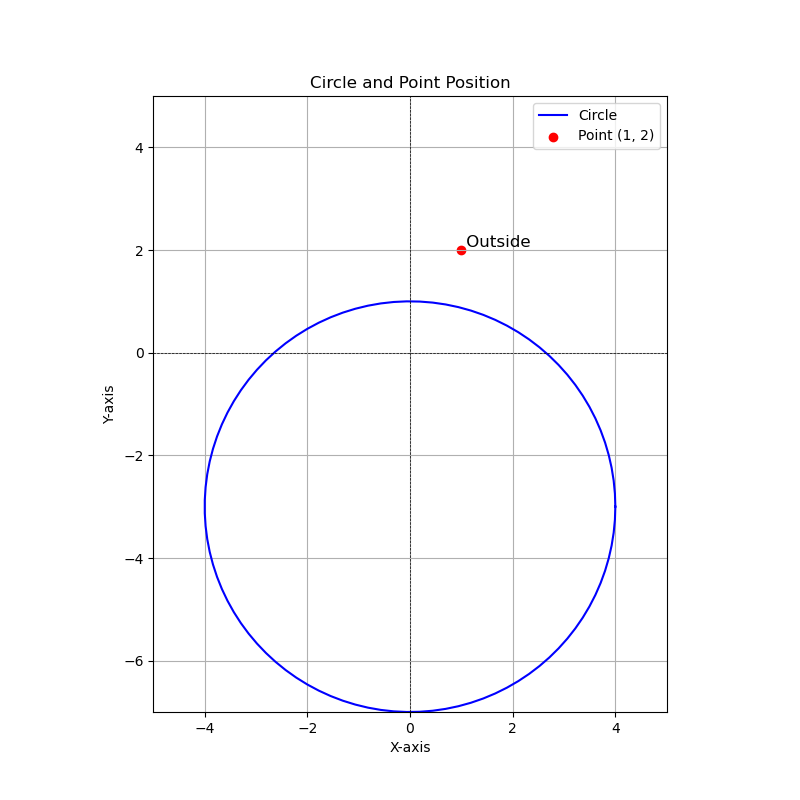
\includegraphics[width=0.7\linewidth]{figure/Figure_1.png} % Ensure this file exists
	\caption{Circle}
\end{figure}

\end{document}

